\documentclass{article}
\usepackage{hyperref}
\usepackage[pdftex]{graphicx}
\usepackage{fullpage}
\begin{document}
\title{User Manual}
\author{PLP Dev Team\\
        ECEN \\
        Oklahoma State University, OK}
        
\maketitle
\pagebreak
\tableofcontents

\section{Introduction}
This document serves as the hardware and software developers guide for the 
Progressive Learning Platform (PLP) System on a Chip. The PLP board is a 
unique learning platform designed to be simple, open, and of course, useful 
for education. 
\section{Getting PLP}
Always make sure to download the latest version of PLP. This manual 
reflects the latest version.

PLP is available for download in the 
\href{http://code.google.com/p/progressive-learning-platform/downloads/list}{downloads}
section. The archive contains the following directory structure:

\begin{enumerate}
\item hw - Hardware images for the CPU
\item sw - Software tools, example programs, and software library
	\begin{enumerate}
	\item PLPTool - PLP Software tools, see next section
	\item libplp - \href{http://code.google.com/p/progressive-learning-platform/wiki/libplp}{PLP software library}
	\item examples - \href{http://code.google.com/p/progressive-learning-platform/wiki/SoftwareExamples}{Software examples}
	\end{enumerate} 
\end{enumerate} 

\section{Software Tools (PLPTool)}
PLPTool is a software suite for PLP that includes an assembler, a simulator, 
and a board programmer interface. 
\subsection{Running PLPTool}
PLPTool requires a 
\href{http://www.oracle.com/technetwork/java/javase/downloads/index.html}{Java Runtime Environment}
that complies with at least Java 2 Platform SE 5 (1.5) specifications. PLPTool 
is shipped with 
\href{http://rxtx.qbang.org/wiki/index.php/Main_Page}{RXTX library}
for serial communication in Windows. If you use Linux, you will have to 
install the library provided by the distribution that you use. Serial 
communication is used to download programs to the board.

PLPTool is located in \verb+sw/PLPTool+ in the PLP download archive. You 
need to uncompress this folder to run the software. If you use Windows, you 
need to run the batch file \verb+PLPToolWin32.bat+ if you use the 32-bit 
version of Windows, or \verb+PLPToolWin64.bat+ if you use the 64-bit version. 
PLPTool will give a 
warning if it can not detect the RXTX library, and the user will not be 
able to program the board or use the serial terminal. 
\subsubsection{Command Line Options}
Launching PLPTool with no command line arguments will launch the GUI. Launching PLPTool with a \verb+.plp+ file as the only argument will launch the GUI and 
open that project.

\begin{verbatim}
java -jar PLPTool.jar <.plp file to open>
\end{verbatim}

or in Windows, where XX is the CPU type (32- or 64-bit):

\begin{verbatim}
PLPToolWinXX.bat <.plp file to open>
\end{verbatim}

Running PLPTool with the command line argument below will list the source files that are in the project. It will also display the index of said source files that is used to export, remove, or set a source file as top level source.

\begin{verbatim}
java -jar PLPTool.jar -plp <plpfile>
\end{verbatim}

The \verb+-plp <plpfile>+ command can also take additional arguments that can be used to manipulate the project file without launching the GUI: 

\begin{tabular}{ | l | l | }
\hline
Command Line Option & Description \\ \hline
-c <asm 1> <asm 2> ... & Creates <plpfile> and imports <asm 1>, <asm 2>, ... to the project \\
-p <port> 	& Programs <plpfile> to serial port <port> \\
-a 	& Performs an assembly of the source files inside <plpfile> \\
-i <asm 1> <asm 2> ... 	& Imports <asm 1>, <asm 2>, ... into <plpfile> project file \\

-d <directory> 	& Imports all files in <directory> to the <plpfile> project file \\
-e <index> <file> 	& Exports the source file with the index <index> as <file> \\
-r <index> 	& Removes the source file with the index <index> \\
-s <index> 	& Set the source file with the index <index> as the main program\\

-m <index> <new index> 	& Set <new index> for the source file with the index <index> \\
\hline
\end{tabular}

\subsection{Graphical User Interface}
PLPTool starts in the development environment view, displaying the current open file, files in the project, and a status window. From this view, you can import or create new assembly files, assemble the project, launch the simulator, and program the PLP board. 

\begin{center}
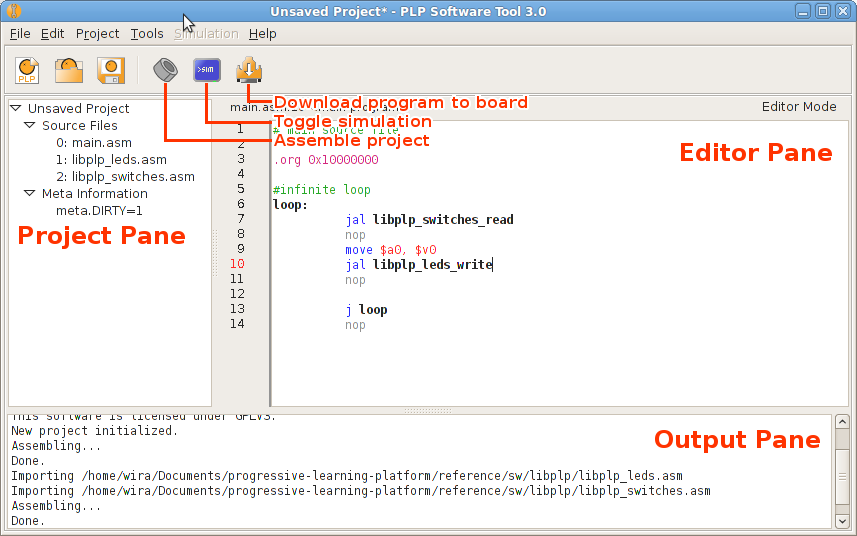
\includegraphics[scale=0.5]{../../images/plptool/plptool30_editor_view.png}
\end{center}

The \textbf{Project Pane} contains all the source files in the project. 
The \textbf{Editor Pane} displays the contents of the currently open source 
file. The \textbf{Output Pane} displays informative, warning, and error 
messages. 
\subsection{Cycle Accurate Simulator}
PLPTool includes a cycle-accurate simulator of the system. This simulator can be accessed from the command-line, or through the graphical user interface. 

\begin{center}
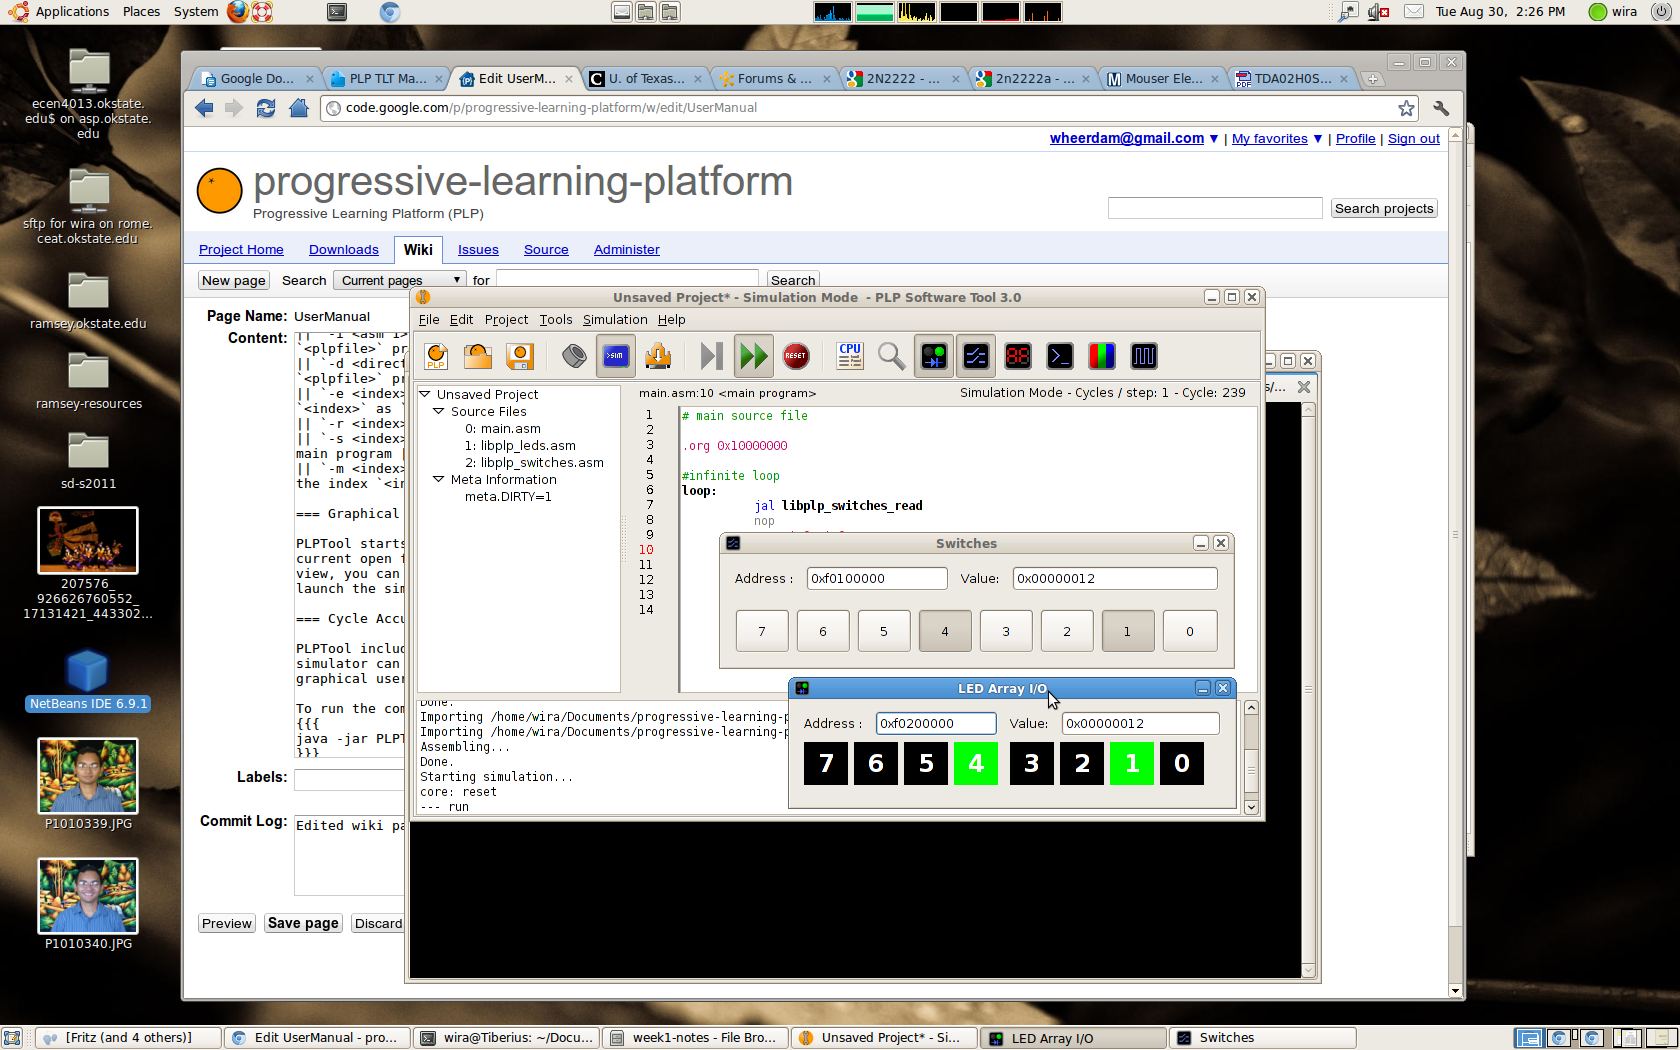
\includegraphics[scale=0.5]{../../images/plptool/plptool30_simulation_mode.png}
\end{center}

The simulation mode adds additional controls to the main window. The first three are the step, run, and reset buttons. Step (F5) will advance the simulation by one cycle, the run toggle button (F7) will continuously run the simulation, and the reset button (F9) will return the CPU to the reset state. The CPU view button will display the CPU window where users can view and modify register file contents, see the disassembly listing, and access the debug console for advanced interaction with the simulation. 
\subsubsection{Setting a Breakpoint}
Breakpoint can be set by double-clicking the line number column. This can only 
applies in lines where there is actually an instruction present. 
Double-click on an existing breakpoint to clear it, or use 
\verb+Tools -> Clear Breakpoints+ to clear ALL breakpoints. 

\subsubsection{Command-Line Mode}
To run the command-line simulator:

\begin{verbatim}
java -jar PLPTool.jar -s <plp file to simulate>
\end{verbatim}
\subsection{Programmer}
You can program the PLP board by selecting 
\verb+Project->Program PLP Board+ 
in the development view. The programmer dialog allows you to select the 
communications port.

Additionally, you can program the PLP board from the command line with:

\begin{verbatim}
java -jar PLPTool.jar -plp <plp project> -p <communications port>
\end{verbatim}
\section{Instruction Set and Assembly Language}
This section describes all supported instructions and pseudo-instructions by the PLP system. It also gives examples on how to use each instruction in a program and notes on limitations. 
\subsection{Syntax}
\subsubsection{Instructions}
Instructions are written in 
\verb+<opcode> <destination>,<operands>+
format, which differ slightly for each type of instruction.

R-type instructions have an opcode and three arguments (either registers or shift amount). For example, to add register 
\verb+$s0+ and \verb+$s1+, 
and store it in register \verb+$t0+, the instruction would be:

\begin{verbatim}
add $t0, $s0, $s1
\end{verbatim}

Shift instructions use the last argument for the shift amount:

\begin{verbatim}
sll $t0, $s0, 5  #shift s0 left 5 bits and store into t0
\end{verbatim}

I-type instructions have two register arguments and an immediate field. For example, to perform a logical OR on 
\verb+$s0+ with the value 0xfeed and store the result in 
\verb+$t0+, the instruction would be:

\begin{verbatim}
ori $t0, $s0, 0xfeed
\end{verbatim}

You may also specify the immediate field in decimal by leaving off the leading '0x'.

Branch instructions require the immediate field to be a label name:

\begin{verbatim}
beq $s0, $s1, loop #if s0 == s1, branch to label "loop"
\end{verbatim}

J-type instructions have only one argument, and must be a label:

\begin{verbatim}
jal my_function #jump and link to label "my_function"
\end{verbatim}

\subsubsection{Pseudo-ops}
PLPTool supports a number of pseudo instructions designed to ease programming and make the assembly more human readable. A list of these instructions, as well as what they map to in the core instruction set is given later in this document. 
\subsubsection{Memory Organization (.org)}
In order to resolve branch and jump targets, the programmer must inform the 
assembler \textbf{before} any instructions, labels, or includes, where the 
program starts in memory. The address must be word aligned (multiple of 4).

\begin{verbatim}
For example, to begin the program at address 0x10000000 (RAM): 
\end{verbatim}

\subsubsection{Labels}
Label support allows the programmer to use branch and jump instructions. Labels are appended with a colon.

For example, to create a label "main": 

\begin{verbatim}
<instructions>
main:
<instructions>
\end{verbatim}

\subsubsection{Comments}
Comments may appear anywhere in the program code, including on label, 
instruction, and directive lines. Comments are prefixed with a \verb+'#'+
character, and all text after the comment character until the end of the line is ignored by the assembler. 

\begin{verbatim}
#a comment on my own line!
add $s0, $s0, $s1 #another comment!
\end{verbatim}

\subsubsection{Data and String Allocation}
There are three ways to allocate space for data with PLPTool: allocating (and optionally initializing) a single word, allocating space in terms of number of words, and by allocating a string. 
\paragraph{Allocate and Initialize Word}
The \verb+.word+ directive allocates a single word with or without an initial 
value. This is especially useful after a label for easy access.

For example, to allocate a variable, initialized to the value 4: 

\begin{verbatim}
my_variable:
.word 4

...

li $t0, my_variable #get a pointer to my variable
lw $t1, 0($t0)      #t1 has my_variable now
\end{verbatim}

\paragraph{Empty Space Allocation}
PLPTool supports allocating space by taking the number of words to allocate, 
as opposed to a single word with the \verb+.word+ directive. This is 
accomplished using the \verb+.space+ directive. For example, to allocate a 
variable with length of 2 words: 

\begin{verbatim}
long_variable:
.space 2

...

li $t0, long_variable #get a pointer to the variable
lw $t1, 0($t0)        #get first word
lw $t2, 4($t0)        #get second word
\end{verbatim}

\paragraph{String Allocation}
PLPTool also supports two types of string allocation
\verb+.ascii, and .asciiz. .ascii+
allocates a packed array of characters without a trailing null 
terminator, which indicates the end of a string.
\verb+.asciiz+ allocates a packed array of characters with a trailing 
null terminator. 

\begin{verbatim}
#a string of characters
my_string:
.ascii "a bunch of characters" #no null terminator here!
#a null terminated string of characters
my_string_null:
.asciiz "a bunch of characters" #null terminated! use me for string operations
\end{verbatim}
PLPTool also supports escaping newline characters with \verb+\n+. 
\subsubsection{Notes on the Assembler}
\verb+.org+ must be the first non-comment statement in the program.

It is possible to load a pointer to a label using the load immediate pseudo instruction (li). 
\subsection{Ops}
\subsubsection{R-type Arithmetic and Logical Instructions}
\subsubsection{R-type Shift Instructions}
\subsubsection{R-type Jump Register Instructions}
\subsubsection{I-type Branch Instructions}
\subsubsection{I-type Arithmetic and Logical Instructions}
\subsubsection{I-type Load Upper Immediate Instruction}
\subsubsection{I-type Load and Store Word Instructions}
\subsubsection{J-type Instructions}
\subsection{Pseudo-ops}
\subsection{Notes on Register Usage}
\section{Hardware Description}
\subsection{Memory Map}
\subsection{ROM}
\subsection{RAM}
\subsection{UART}
\subsection{Switches}
\subsection{LEDs}
\subsection{GPIO}
\subsection{VGA}
\subsection{PLPID}
\subsection{Timer}
\subsection{Seven Segment}
\subsection{Interrupt Controller}
\subsection{Performance Counters}
\section{Bootloader (fload)}
\end{document}
